\documentclass[11pt,a4paper]{article}
\usepackage{booktabs}
\usepackage{multicol}
\usepackage{titlesec}
\usepackage{fancyhdr}
\usepackage{notes}
\usepackage{tikz}

\hypersetup{colorlinks=true, linkcolor=blue, urlcolor=blue, citecolor=blue}
\setlist[itemize]{leftmargin=*}
\setlist[enumerate]{leftmargin=*}

\pagestyle{fancy}
\fancyhf{}
\lhead{Geophysics IIIA: Potential Fields \& Geothermics}
\rhead{Week 4 Components Library}
\cfoot{\thepage}

\title{Week 4 --- Superposition Component Library}
\author{Geophysics 3A: Potential Fields \& Geothermics}
\date{\today}

\begin{document}
\maketitle
\vspace{-1em}

\section*{How to use}
Select 2--3 components to build a plausible local cross-section. For each, choose a realistic $\Delta\rho$ (from Density Worksheet), depth, and width. Overlay normalized response shapes, scale amplitudes, shift laterally, and \emph{sum} to obtain a composite gravity profile.

\begin{multicols}{2}
\subsection*{A) Basement Step with Sedimentary Wedge}
\begin{itemize}
  \item \textbf{Geology:} Sediments thickening toward a normal fault; basement uplift on one side.
  \item \textbf{Kernel:} Edge-dominated (polygon/step); asymmetry likely.
  \item \textbf{Params:} $\Delta\rho$ (sediment vs.\ basement): $\sim$200--600 kg m$^{-3}$; depth to top: 0.5--2 km; wedge width: 1--5 km.
\end{itemize}
\begin{center}
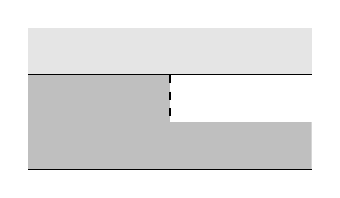
\begin{tikzpicture}[scale=0.6]
\fill[gray!20] (-3,0) rectangle (3,1);
\fill[gray!50] (-3,-2) -- (-3,0) -- (0,0) -- (0,-1) -- (3,-1) -- (3,-2) -- cycle;
\draw (-3,0) -- (3,0); \draw (-3,-2) -- (3,-2);
\draw[dashed] (0,0) -- (0,-1);
\end{tikzpicture}
\end{center}

\subsection*{B) Mafic Dike (2D Cylinder Proxy)}
\begin{itemize}
  \item \textbf{Geology:} Narrow, dense intrusive cutting felsic country rock.
  \item \textbf{Kernel:} Narrow positive peak; half-width gives depth cue.
  \item \textbf{Params:} $\Delta\rho$ (mafic--felsic): $\sim$200--400 kg m$^{-3}$; width: 50--300 m; depth to top: 0.1--1 km.
\end{itemize}
\begin{center}
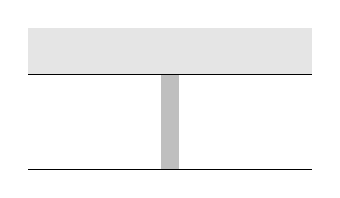
\begin{tikzpicture}[scale=0.6]
\fill[gray!20] (-3,0) rectangle (3,1);
\fill[gray!50] (-0.2,0) -- (0.2,0) -- (0.2,-2) -- (-0.2,-2) -- cycle;
\draw (-3,0) -- (3,0); \draw (-3,-2) -- (3,-2);
\end{tikzpicture}
\end{center}

\subsection*{C) Felsic Pluton (Broad Polygon)}
\begin{itemize}
  \item \textbf{Geology:} Large, less dense body emplaced at depth.
  \item \textbf{Kernel:} Broad, low-amplitude positive or negative depending on host; gentle gradients.
  \item \textbf{Params:} $\Delta\rho$: $-100$ to $+200$ kg m$^{-3}$; width: 2--10 km; depth to top: 1--5 km.
\end{itemize}
\begin{center}
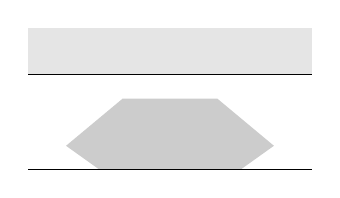
\begin{tikzpicture}[scale=0.6]
\fill[gray!20] (-3,0) rectangle (3,1);
\fill[gray!40] (-2.2,-1.5) -- (-1.0,-0.5) -- (1.0,-0.5) -- (2.2,-1.5) -- (1.5,-2) -- (-1.5,-2) -- cycle;
\draw (-3,0) -- (3,0); \draw (-3,-2) -- (3,-2);
\end{tikzpicture}
\end{center}

\subsection*{D) Regolith/Weathered Cap (Thin Negative Slab)}
\begin{itemize}
  \item \textbf{Geology:} Near-surface low-density layer.
  \item \textbf{Kernel:} Thin slab; small, relatively localized negative anomaly.
  \item \textbf{Params:} $\Delta\rho$: $-100$ to $-400$ kg m$^{-3}$; thickness: 5--50 m; lateral extent: 0.5--2 km.
\end{itemize}
\begin{center}

\begin{tikzpicture}[scale=0.6]
\fill[gray!20] (-3,0) rectangle (3,1);
\fill[white] (-3,0) rectangle (3,0.2);
\draw (-3,0) -- (3,0); \draw (-3,-2) -- (3,-2);
\end{tikzpicture}
\end{center}
\end{multicols}

\section*{Notes}
Use the \emph{Formula Sheet} for scale/shape cues (half-width, edge effects) and superposition rules. Combine components judiciously to avoid overfitting.

\end{document}